% !TeX program = xelatex
% !TeX options = -shell-escape -synctex=1 -interaction=nonstopmode -file-line-error "%DOC%"
\documentclass[aspectratio=169,11pt]{beamer}

% ———- голый beamer ———-
\setbeamertemplate{navigation symbols}{}
\setbeamertemplate{headline}{}
\setbeamertemplate{footline}{}
\setbeamertemplate{frametitle}{}
\setbeamersize{text margin left=0pt, text margin right=0pt}

\usepackage{fontspec}
\setmainfont{Inter}[Ligatures=TeX]
\setsansfont{Inter}[Ligatures=TeX]
\newfontfamily\InterBold{Inter Bold}[Ligatures=TeX]
\newfontfamily\InterSemi{Inter SemiBold}[Ligatures=TeX]

\usepackage{tikz}
\usetikzlibrary{arrows.meta,positioning,calc}
\usepackage{graphicx}
\usepackage{booktabs}
\usepackage{array}
\usepackage{colortbl}
\usepackage{hhline}
\usepackage{tabularx}

\newcolumntype{L}[1]{>{\raggedright\arraybackslash}m{#1}}
\newcolumntype{C}[1]{>{\centering\arraybackslash}m{#1}}

% ———- палитра М.Видео ———-
\definecolor{mvred}{HTML}{F20601}
\definecolor{mvdark}{HTML}{1C1C1E}
\definecolor{mvgray}{HTML}{6E6E73}
\definecolor{cardbg}{HTML}{F5F5F6}
\definecolor{pinkband}{HTML}{FDECEC}
\definecolor{okgreen}{HTML}{1F8A50}
\definecolor{warnorange}{HTML}{C75000}
\definecolor{purpletag}{HTML}{6A35B0}

\graphicspath{{assets/}{assets/icons/}{../figures/}{figures/}{../figures/complex_eda/}{../figures/complex_eda/markov/}{../figures/complex_eda/model_tag/}{../figures/preprocessing/}{../figures/apps/}}

% ———- макро ———-
\newcommand{\kicker}[1]{{\color{mvred}\InterBold\fontsize{8}{10}\selectfont\MakeUppercase{#1}}}
\newcommand{\slidetitle}[1]{{\color{mvdark}\InterBold\fontsize{15.5}{18}\selectfont #1}}

% розовый блок с меткой (метка настраивается — не всегда «вывод»)
\newcommand{\pinknote}[2]{%
  \begin{tikzpicture}
    \node[fill=pinkband, rounded corners=2pt, inner xsep=9pt, inner ysep=5.5pt,
          text width=\dimexpr\textwidth-18pt\relax] {%
      {\color{mvred}\InterBold\fontsize{8}{10}\selectfont #1}\hspace{7pt}{\color{mvdark}\fontsize{8.5}{11}\selectfont #2}};
  \end{tikzpicture}}
\newcommand{\conclusion}[1]{\pinknote{ВЫВОД}{#1}}

% серый информационный блок
\newcommand{\graynote}[2]{%
  \begin{tikzpicture}
    \node[fill=cardbg, rounded corners=2pt, inner xsep=9pt, inner ysep=5.5pt,
          text width=\dimexpr\textwidth-18pt\relax] {%
      {\color{mvdark}\InterBold\fontsize{8}{10}\selectfont #1}\hspace{7pt}{\color{mvdark}\fontsize{8.5}{11}\selectfont #2}};
  \end{tikzpicture}}

\newcommand{\numdot}[1]{%
  \tikz[baseline=-0.6ex]{\node[circle, fill=mvred, text=white, inner sep=1pt, minimum size=12pt, font=\InterBold\fontsize{7}{8}\selectfont]{#1};}}

\newcommand{\cornerlogo}{%
  \begin{tikzpicture}[remember picture, overlay]
    \node[anchor=north east, xshift=-0.5cm, yshift=-0.38cm] at (current page.north east)
      {
\includegraphics[height=0.85cm]{m_letter.png}};
  \end{tikzpicture}}

\newcommand{\slidehead}[2]{%
  \cornerlogo
  \vspace{0.38cm}\par
  \hspace{0.85cm}\begin{minipage}{\dimexpr\paperwidth-1.7cm\relax}
  \kicker{#1}\par\vspace{3pt}
  \slidetitle{#2}\par\vspace{7pt}}
\newcommand{\slidefoot}{\end{minipage}}

\newcommand{\bodytext}{\fontsize{8.5}{11.5}\selectfont}
\newcommand{\smalltext}{\fontsize{7.5}{10}\selectfont}

% таблицы
\definecolor{tblline}{HTML}{DDDDDD}
\arrayrulecolor{tblline}
\newcommand{\ttext}{\fontsize{7}{9}\selectfont}
\newcommand{\thead}[1]{\cellcolor{mvdark}{\color{white}\InterSemi\ttext #1}}
\newcommand{\theadl}[1]{\cellcolor{mvdark}{\color{white}\InterSemi\ttext #1}}
\newcommand{\tacc}[1]{\cellcolor{mvred}{\color{white}\InterSemi\ttext #1}}
\newcommand{\tcellc}[1]{{\ttext\color{mvdark}#1}}
\newcommand{\tcelll}[1]{{\ttext\color{mvdark}#1}}
\newcommand{\hnum}[1]{{\InterBold\color{mvdark}#1}}
\newcommand{\hb}[1]{{\InterSemi\color{mvdark}#1}}
\newcommand{\tnote}[1]{{\color{mvred}\itshape\fontsize{7}{9}\selectfont #1}}

% чипы-подсветка слов (пример разметки прямо в строке)
\newcommand{\wtag}[2]{\tikz[baseline=-0.55ex]{\node[rounded corners=2pt, fill=#1, inner xsep=4pt, inner ysep=2.2pt, font=\InterSemi\fontsize{7.8}{9}\selectfont, text=white]{#2};}}
\newcommand{\wplain}[1]{\tikz[baseline=-0.55ex]{\node[rounded corners=2pt, fill=cardbg, inner xsep=4pt, inner ysep=2.2pt, font=\fontsize{7.8}{9}\selectfont, text=mvdark]{#1};}}
\newcommand{\biotag}[2]{\tikz[baseline=-0.55ex]{\node[rounded corners=1.5pt, fill=#1, inner xsep=2.5pt, inner ysep=1pt, font=\fontsize{6.5}{7.5}\selectfont\color{white}]{#2};}}

% ———- жирный шеврон, как в шаблоне М.Тех (стрелка-галка) ———-
\newcommand{\chevron}{%
  \raisebox{-0.55ex}{
\begin{tikzpicture}
    \draw[mvred, line width=2.6pt, line cap=round, line join=round]
      (0,0.30) -- (0.15,0.15) -- (0,0);
  \end{tikzpicture}}}
% шаг пайплайна: #1 fill, #2 text color, #3 текст
\newcommand{\pipestep}[3]{%
  \begin{tikzpicture}[baseline=(b.center)]
    \node[fill=#1, rounded corners=3pt, minimum height=1.15cm, text width=1.85cm,
          align=center, inner sep=3pt, font=\InterSemi\fontsize{7.5}{9}\selectfont, text=#2] (b) {#3};
  \end{tikzpicture}}
\newcommand{\pipestepc}[3]{%
  \begin{tikzpicture}[baseline=(b.center)]
    \node[fill=#1, rounded corners=3pt, minimum height=1.1cm, text width=1.62cm,
          align=center, inner sep=3pt, font=\InterSemi\fontsize{7}{8.5}\selectfont, text=#2] (b) {#3};
  \end{tikzpicture}}
% узкий шаг (6 блоков в ряд)
\newcommand{\pipestepq}[3]{%
  \begin{tikzpicture}[baseline=(b.center)]
    \node[fill=#1, rounded corners=3pt, minimum height=0.88cm, text width=1.42cm,
          align=center, inner sep=2.5pt, font=\InterSemi\fontsize{6.6}{8}\selectfont, text=#2] (b) {#3};
  \end{tikzpicture}}
% карточка с иконкой
\newcommand{\iconcard}[3]{%
  \begin{tikzpicture}
    \node[fill=cardbg, rounded corners=4pt, inner sep=6pt, text width=2.7cm, align=center,
          minimum height=2.05cm, anchor=north] (c) {%
      \includegraphics[height=0.68cm]{#1}\par\vspace{3pt}
      {\InterSemi\fontsize{7.5}{9.5}\selectfont\color{mvdark}#2}\par\vspace{2pt}
      {\fontsize{6.4}{8}\selectfont\color{mvgray}#3}};
  \end{tikzpicture}}

\setlength{\parskip}{0pt}

\begin{document}

% ============================================================
% 1. ТИТУЛ
% ============================================================
\begin{frame}[plain]
\begin{tikzpicture}[remember picture, overlay]
  \fill[mvred] (current page.south west) rectangle (current page.north east);
  \node[anchor=east, inner sep=0pt] at ([xshift=0.32\paperwidth]current page.east)
    {
\includegraphics[height=1.06\paperheight]{kurs1_image1.png}};
  \node[anchor=west, align=left] at ([xshift=0.9cm, yshift=2.05cm]current page.west)
    {\color{white}\InterBold\fontsize{10}{12}\selectfont ДЕНЬ 03 · БУТКЕМП М.ВИДЕО · NLP / SEARCH};
  \node[anchor=west, align=left] at ([xshift=0.88cm, yshift=0.9cm]current page.west)
    {\color{white}\InterBold\fontsize{27}{31}\selectfont Глубокий EDA};
  \node[anchor=west, align=left] at ([xshift=0.88cm, yshift=-0.05cm]current page.west)
    {\color{white}\InterBold\fontsize{27}{31}\selectfont и первый MVP};
  \node[anchor=west, align=left, text width=0.5\paperwidth] at ([xshift=0.9cm, yshift=-1.9cm]current page.west)
    {\color{white}\fontsize{11}{15}\selectfont Предобработка, тег MODEL, разбор схем разметки, рабочий каскад моделей и два готовых приложения: умный поиск и разметка для команды.};
  \node[anchor=south west] at ([xshift=0.9cm, yshift=0.5cm]current page.south west)
    {\color{white}\fontsize{9}{11}\selectfont Умный поиск · Понимание запроса · MVP};
\end{tikzpicture}
\end{frame}

% ============================================================
% 2. ЧТО СДЕЛАЛИ КО ДНЮ 3
% ============================================================
\begin{frame}[t]
\slidehead{день 03 · итоги}{Что собрали ко Дню 3}
\pinknote{КОРОТКО}{За день прошли путь от анализа данных до работающего продукта: единая предобработка, новый тег MODEL, каскад из трёх обученных моделей и два настольных приложения.}
\vspace{22pt}\par
\begin{center}
\begin{tikzpicture}[node distance=12pt]
  \node (o1) {\iconcard{ic_tools.png}{Предобработка}{чистка, расклейка склеек, словарь моделей на 6130 фраз}};
  \node[right=of o1] (o2) {\iconcard{ic_chat.png}{Схемы разметки}{разобрали IO, BIO, BILOU — храним спаны, учим на BIO}};
  \node[right=of o2] (o3) {\iconcard{ic_rocket.png}{Модели MVP}{классификатор бренда, CRF, марковский типизатор}};
  \node[right=of o3] (o4) {\iconcard{ic_dev.png}{Приложения}{умный поиск + разметка для команды (3 сборки)}};
\end{tikzpicture}
\end{center}
\slidefoot
\end{frame}

% ============================================================
% 3. ГЛУБОКИЙ EDA — МАСШТАБ И ДЛИНЫ
% ============================================================
\begin{frame}[t]
\slidehead{глубокий eda · данные}{С чем работаем: масштаб и длины}
\begin{columns}[T]
\column{0.5\textwidth}
\vspace{2pt}\centering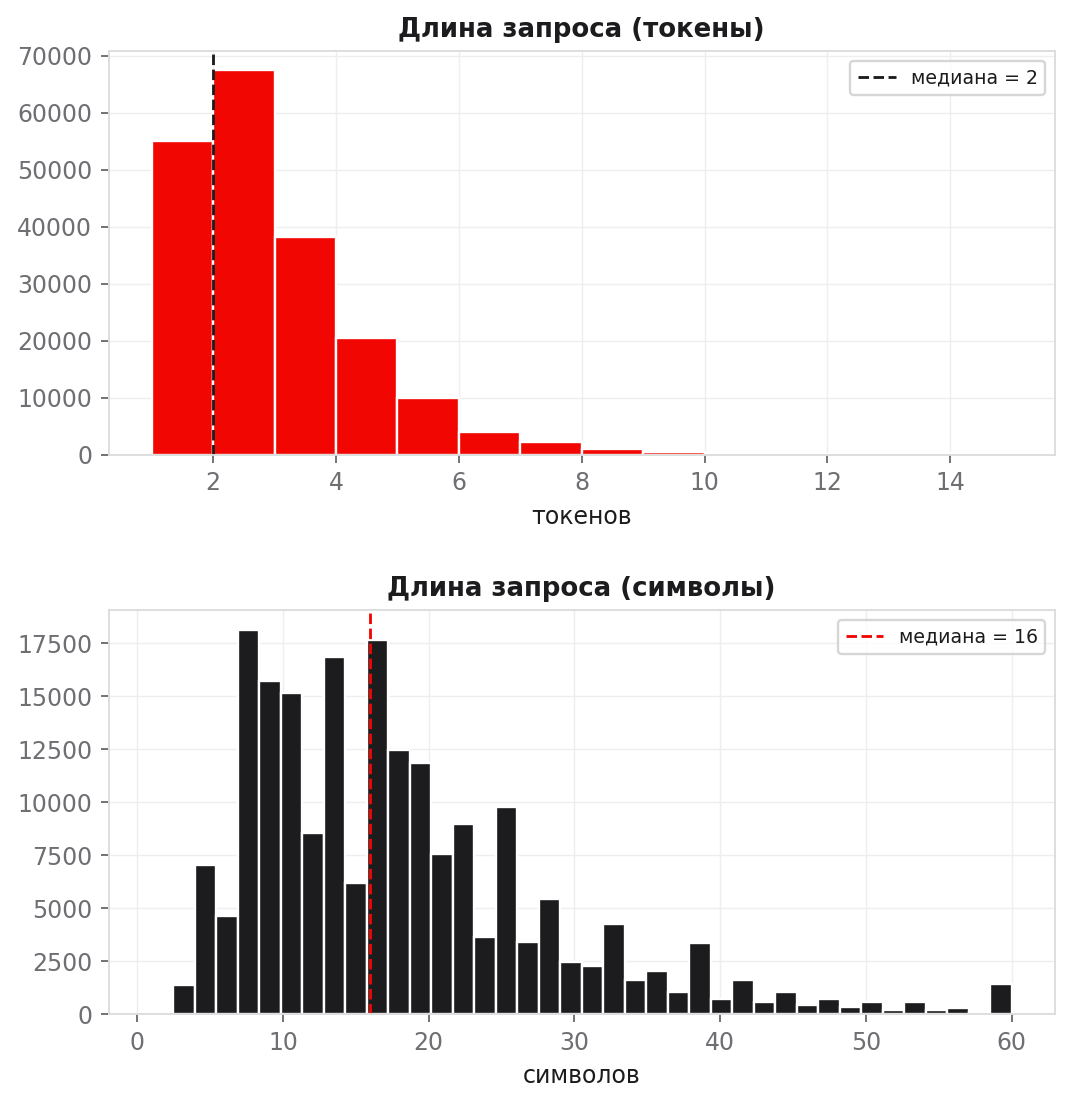
\includegraphics[width=0.98\textwidth,height=4.5cm,keepaspectratio]{01_query_length.png}
\column{0.47\textwidth}
\conclusion{Запросы очень короткие: половина — 2 токена, 99\% укладываются в 7. Это задача понимания запроса, а не разбора длинного документа.}
\vspace{6pt}\par
{\smalltext
\numdot{1}\ 30{,}99 млн кликов, 1{,}18 млн карточек. В семпле 200 тысяч строк — 49 тысяч уникальных запросов и 3{,}1 тысячи брендов.\par\vspace{4pt}
\numdot{2}\ Длина в токенах: медиана 2, у 90\% — до 4, у 99\% — до 7. В символах: 17 и 31.\par\vspace{4pt}
\numdot{3}\ Медианная цена клика — 16 165 ₽, пропусков в ключевых полях нет. Короткие запросы — значит CRF успеет отработать с запасом по времени.}
\end{columns}
\slidefoot
\end{frame}

% ============================================================
% 4. EDA — БРЕНД НЕ В ТЕКСТЕ
% ============================================================
\begin{frame}[t]
\slidehead{глубокий eda · бренды}{73\% брендов нет в тексте запроса}
\begin{columns}[T]
\column{0.5\textwidth}
\vspace{2pt}\centering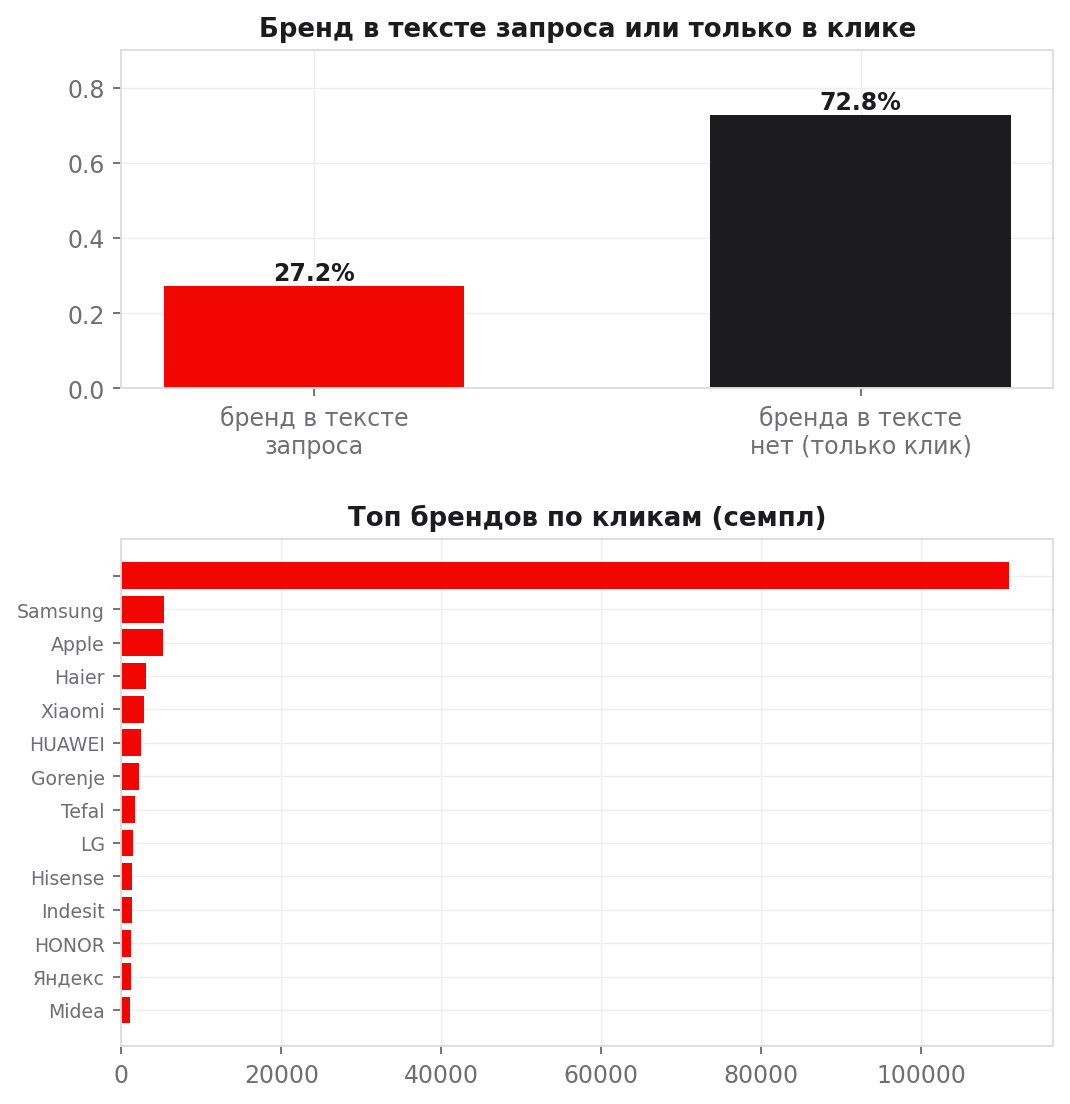
\includegraphics[width=0.98\textwidth,height=4.5cm,keepaspectratio]{04_brand_in_query_vs_click.png}
\column{0.47\textwidth}
\pinknote{ГЛАВНОЕ ЧИСЛО}{Лишь в 27\% кликов бренд написан в самом запросе. В остальных 73\% бренд известен только из кликнутой карточки — словарём его не достать.}
\vspace{6pt}\par
{\smalltext
\numdot{1}\ Пользователь пишет «айфон 15» — слова «Apple» нет, но купить он хочет именно Apple. Поэтому нужен классификатор бренда по всему запросу.\par\vspace{4pt}
\numdot{2}\ 17\% запросов кликают по двум и более брендам — берём самый частый бренд с весом по позиции клика.\par\vspace{4pt}
\numdot{3}\ Там, где словарь нашёл бренд в тексте, он совпадает с брендом клика в 79{,}5\% случаев — сигналы согласованы, можно учить общую модель.}
\end{columns}
\slidefoot
\end{frame}

% ============================================================
% 5. EDA — СЛАБАЯ РАЗМЕТКА
% ============================================================
\begin{frame}[t]
\slidehead{глубокий eda · разметка}{Слабая разметка: покрытие и границы}
\begin{columns}[T]
\column{0.5\textwidth}
\vspace{2pt}\centering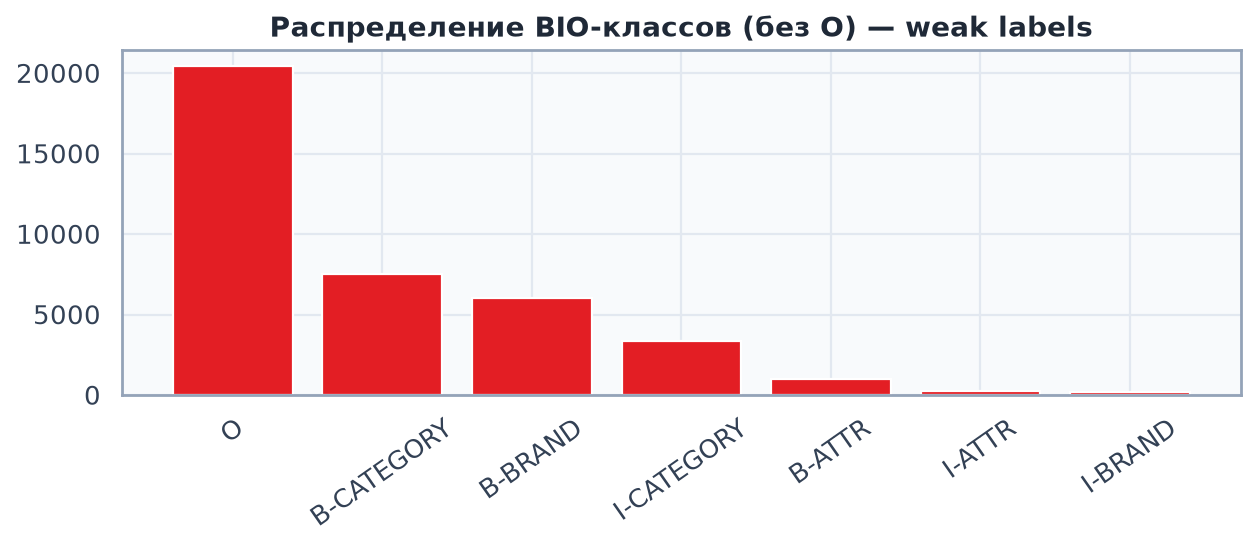
\includegraphics[width=0.98\textwidth,height=4.5cm,keepaspectratio]{03_bio_class_distribution.png}
\column{0.47\textwidth}
\graynote{КАК ЧИТАТЬ}{Слабая разметка — это автоматические теги от словарей и правил. Она бесплатная, но шумная: на ней учим, а проверяем на ручной.}
\vspace{6pt}\par
{\smalltext
\numdot{1}\ Хотя бы одну сущность получают 79{,}8\% запросов: бренд — у 46\%, категория — у 59\%, атрибуты — только у 7\%.\par\vspace{4pt}
\numdot{2}\ У 27\% запросов есть продолжение сущности (теги I) — значит нужны именно границы спанов, а не классификация всего запроса.\par\vspace{4pt}
\numdot{3}\ Регулярки по атрибутам покрывают всего 3\% запросов — атрибуты одним правилом не закрыть, нужен типизатор поверх найденного спана.}
\end{columns}
\slidefoot
\end{frame}

% ============================================================
% 6. ПРЕПРОЦЕССИНГ — ШАГИ (компактно, без вылетов)
% ============================================================
\begin{frame}[t]
\slidehead{предобработка · пайплайн}{Единый слой очистки запроса}
\begin{columns}[T]
\column{0.52\textwidth}
{\InterSemi\fontsize{8.5}{10.5}\selectfont Шесть шагов очистки}\par\vspace{5pt}
{\renewcommand{\arraystretch}{1.22}\setlength{\tabcolsep}{5pt}
\begin{tabular}{|L{2.4cm}|L{4.2cm}|}
\hline
\theadl{Шаг} & \theadl{Что делает}\\
\hline
\tcelll{\hb{Базовая чистка}} & \tcelll{убирает мусорные пробелы, ё $\to$ е}\\
\hline
\tcelll{\hb{Расклейка}} & \tcelll{«128гб» $\to$ «128 гб»}\\
\hline
\tcelll{\hb{Сепараторы}} & \tcelll{«g-pro» $\to$ «g pro»}\\
\hline
\tcelll{\hb{Нормализация}} & \tcelll{единый ключ для словарей}\\
\hline
\tcelll{\hb{Защита брендов}} & \tcelll{«Красный Октябрь» — не цвет}\\
\hline
\tcelll{\hb{Подсказки}} & \tcelll{спаны моделей поверх разметки}\\
\hline
\end{tabular}}
\column{0.46\textwidth}
{\InterSemi\fontsize{8.5}{10.5}\selectfont Зачем один общий слой}\par\vspace{5pt}
{\smalltext
\numdot{1}\ Раньше каждый ноутбук чистил запрос по-своему — результаты не сходились. Теперь очистка одна на всех.\par\vspace{4pt}
\numdot{2}\ Регистр сохраняем там, где он несёт смысл: «красный» — это цвет, а «Красный Октябрь» — бренд конфет.\par\vspace{4pt}
\numdot{3}\ Модуль отдаёт и чистый текст, и подсказки: где в запросе модель, а где защищённый бренд.}
\par\vspace{8pt}
\pinknote{ЭФФЕКТ}{Спан модели появляется у 18\% запросов, склейки чинятся у 11\%, а каждый четвёртый «пустой» хвост после бренда оживает.}
\end{columns}
\slidefoot
\end{frame}

% ============================================================
% 7. НОВЫЙ: ПРИМЕР ПРЕДОБРАБОТКИ С ПОДСВЕТКОЙ
% ============================================================
\begin{frame}[t]
\slidehead{предобработка · пример}{Живой пример: запрос до и после}
\graynote{ИСХОДНЫЙ ЗАПРОС}{«Наушники Logitech G-Pro X SE 128гб» — так пишет реальный пользователь: дефисы, склейки, смесь языков.}
\vspace{10pt}\par
{\InterSemi\fontsize{8.5}{10.5}\selectfont Шаг 1 · расклейка и сепараторы}\par\vspace{4pt}
{\fontsize{9}{13}\selectfont
\wplain{наушники} \ \wplain{logitech} \ \wplain{g} \ \wplain{pro} \ \wplain{x} \ \wplain{se} \ \wplain{128} \ \wplain{гб}}\par\vspace{2pt}
{\smalltext\color{mvgray} «G-Pro» распался в «g pro», «128гб» — в «128 гб». Теперь словари смогут найти каждую часть.}
\par\vspace{10pt}
{\InterSemi\fontsize{8.5}{10.5}\selectfont Шаг 2 · разметка со словарями и подсказками}\par\vspace{4pt}
{\fontsize{9}{13}\selectfont
\wtag{mvred}{наушники · КАТЕГОРИЯ} \ \wtag{mvdark}{logitech · БРЕНД} \ \wtag{okgreen}{g pro x se · МОДЕЛЬ} \ \wtag{warnorange}{128 гб · АТРИБУТ}}\par\vspace{2pt}
{\smalltext\color{mvgray} «g pro x se» поймал словарь моделей (собрали его майнингом — следующие слайды), «128 гб» — регулярка памяти.}
\par\vspace{10pt}
{\InterSemi\fontsize{8.5}{10.5}\selectfont Шаг 3 · готовые факты}\par\vspace{4pt}
{\smalltext бренд = Logitech · категория = наушники · модель = g pro x se · память = 128 ГБ. Именно эти факты дальше идут в поиск и ранжирование.}
\slidefoot
\end{frame}

% ============================================================
% 8. ПРЕПРОЦЕССИНГ — ЭФФЕКТ (график)
% ============================================================
\begin{frame}[t]
\slidehead{предобработка · измерение}{Что даёт предобработка на семпле}
\begin{columns}[T]
\column{0.5\textwidth}
\vspace{2pt}\centering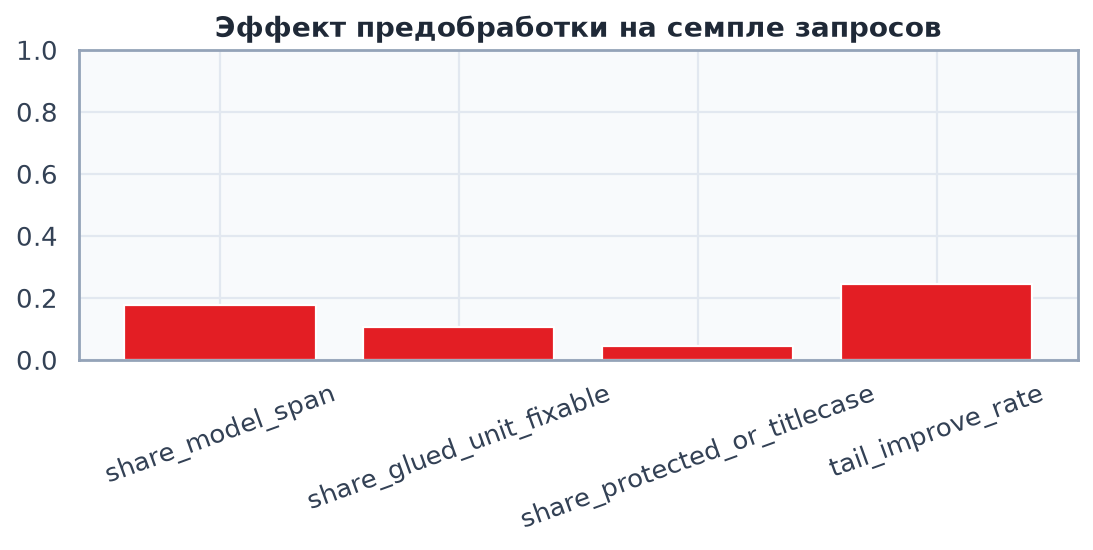
\includegraphics[width=0.98\textwidth,height=4.4cm,keepaspectratio]{02_preprocess_effect.png}
\column{0.47\textwidth}
\graynote{КАК МЕРИЛИ}{Взяли 12 000 уникальных запросов и прогнали через пайплайн дважды: со словарём моделей и без него.}
\vspace{6pt}\par
{\smalltext
\numdot{1}\ 18\% запросов получают спан модели — примерно каждый пятый.\par\vspace{4pt}
\numdot{2}\ 11\% содержат склейку вида «128гб», которую чинит расклейка.\par\vspace{4pt}
\numdot{3}\ 24\% полностью пустых хвостов после бренда получают тег модели после наложения подсказок.\par\vspace{4pt}
\numdot{4}\ Защита брендов и заглавных букв срабатывает у 4{,}5\% — редко, но именно она спасает «Красный Октябрь» от превращения в цвет.}
\end{columns}
\slidefoot
\end{frame}

% ============================================================
% 9. ТЕГ MODEL — ПРОБЛЕМА (новый график)
% ============================================================
\begin{frame}[t]
\slidehead{тег model · проблема}{Хвост после бренда теряется}
\begin{columns}[T]
\column{0.54\textwidth}
\vspace{2pt}\centering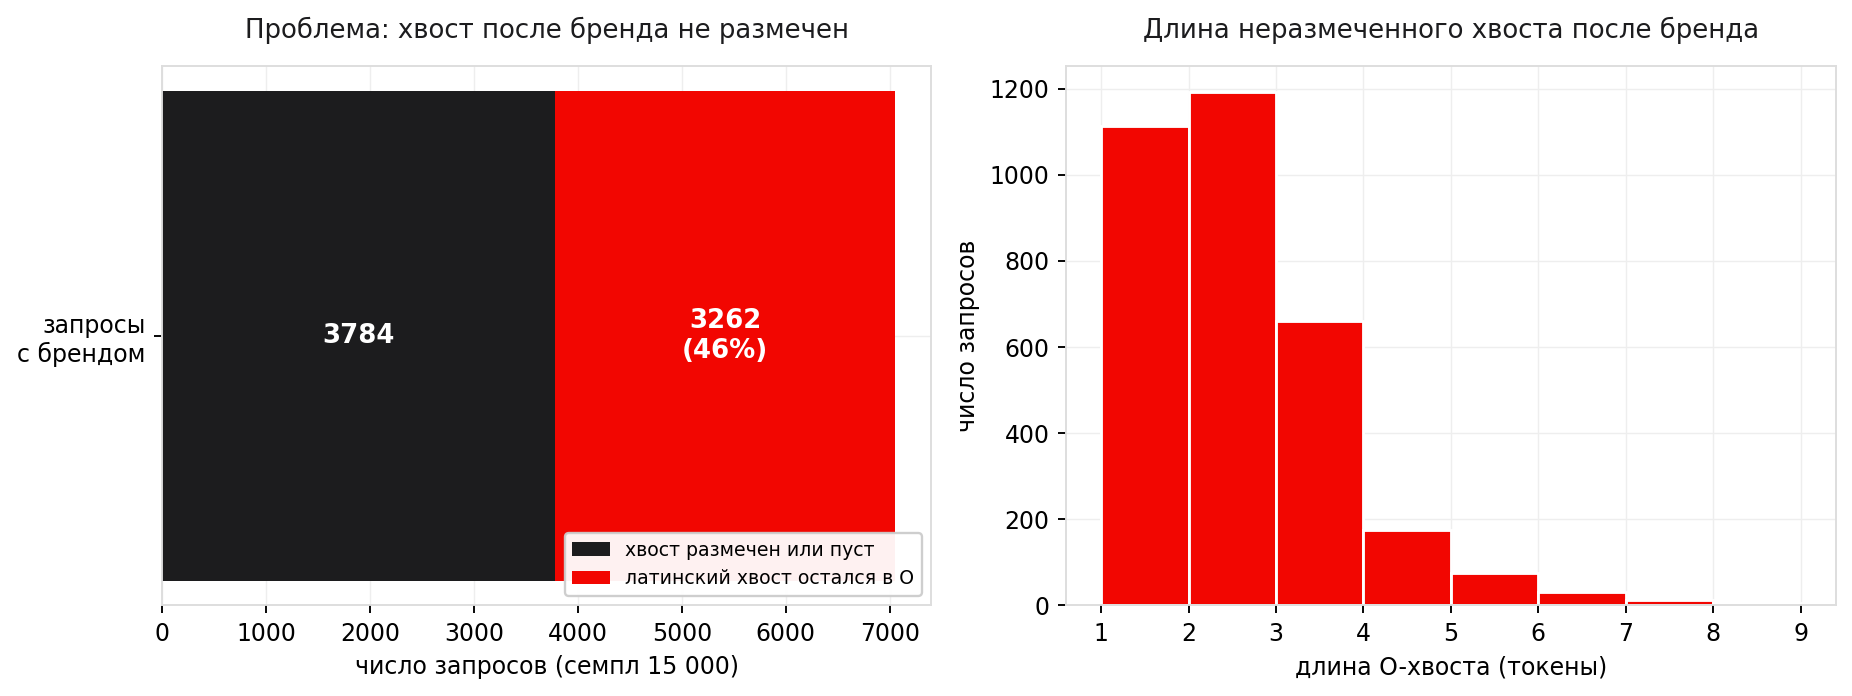
\includegraphics[width=0.98\textwidth,height=4.3cm,keepaspectratio]{model_tag/01_missing_model_problem.png}
\column{0.43\textwidth}
\pinknote{ПРОБЛЕМА}{После бренда часто идёт название линейки — «dyson v15», «galaxy s24». При слабой разметке эти слова остаются без тега, и CRF не может их выучить.}
\vspace{6pt}\par
{\smalltext
\numdot{1}\ Из 15 тысяч запросов бренд есть у 7046. Почти у половины из них (46\%) после бренда остался неразмеченный латинский хвост.\par\vspace{4pt}
\numdot{2}\ Типичная длина хвоста — два токена: «zenbook a16», «ipad air».\par\vspace{4pt}
\numdot{3}\ Это не атрибут — нет числа с единицей измерения. Нужен отдельный тег MODEL и словарь линеек.}
\end{columns}
\slidefoot
\end{frame}

% ============================================================
% 10. НОВЫЙ: ПРИМЕРЫ ПОТЕРЯННЫХ ХВОСТОВ С ПОДСВЕТКОЙ
% ============================================================
\begin{frame}[t]
\slidehead{тег model · примеры}{Как выглядят потерянные хвосты}
\graynote{ДО СЛОВАРЯ}{Серые слова — то, что разметка не смогла объяснить. Именно они и есть модели.}
\vspace{7pt}\par
\begin{columns}[T]
\column{0.48\textwidth}
{\InterSemi\fontsize{8}{10}\selectfont До: хвост без тега}\par\vspace{5pt}
{\fontsize{8.2}{14}\selectfont
\wtag{mvred}{пылесос} \ \wtag{mvdark}{dyson} \ \wplain{v15}\par\vspace{4pt}
\wtag{mvred}{телефон} \ \wtag{mvdark}{samsung} \ \wplain{galaxy} \ \wplain{s24}\par\vspace{4pt}
\wtag{mvdark}{asus} \ \wplain{zenbook} \ \wplain{a16}\par\vspace{4pt}
\wtag{mvdark}{apple} \ \wplain{ipad} \ \wplain{air}}
\column{0.5\textwidth}
{\InterSemi\fontsize{8}{10}\selectfont После: словарь линеек подключён}\par\vspace{5pt}
{\fontsize{8.2}{14}\selectfont
\wtag{mvred}{пылесос} \ \wtag{mvdark}{dyson} \ \wtag{okgreen}{v15 · МОДЕЛЬ}\par\vspace{4pt}
\wtag{mvred}{телефон} \ \wtag{mvdark}{samsung} \ \wtag{okgreen}{galaxy s24 · МОДЕЛЬ}\par\vspace{4pt}
\wtag{mvdark}{asus} \ \wtag{okgreen}{zenbook a16 · МОДЕЛЬ}\par\vspace{4pt}
\wtag{mvdark}{apple} \ \wtag{okgreen}{ipad air · МОДЕЛЬ}}
\end{columns}
\vspace{10pt}\par
\pinknote{ЧТО ИЗМЕНИЛОСЬ}{Хвост после бренда перестал быть «мусором» — теперь это полноценный факт «модель», по которому можно искать и ранжировать.}
\slidefoot
\end{frame}

% ============================================================
% 11. МАЙНИНГ СЛОВАРЯ — КАК РАБОТАЕТ (пример g pro)
% ============================================================
\begin{frame}[t]
\slidehead{тег model · майнинг}{Майнинг словаря: пример «g pro»}
\graynote{ИДЕЯ}{Названия кликнутых карточек уже содержат модели. Находим в названии бренд — и всё, что идёт после него, считаем кандидатом в модели.}
\vspace{8pt}\par
\begin{columns}[T]
\column{0.55\textwidth}
{\InterSemi\fontsize{8.5}{10.5}\selectfont Название карточки $\to$ кандидаты}\par\vspace{5pt}
{\fontsize{8.5}{12}\selectfont
\wplain{Наушники} \ \wtag{mvdark}{Logitech} \ \wtag{okgreen}{G} \ \wtag{okgreen}{PRO} \ \wtag{okgreen}{X} \ \wtag{okgreen}{SE} \ \wplain{Black}}\par\vspace{6pt}
{\smalltext После бренда снимаем от одного до четырёх коротких токенов и получаем цепочку кандидатов:}\par\vspace{4pt}
{\renewcommand{\arraystretch}{1.2}\setlength{\tabcolsep}{6pt}
\begin{tabular}{|L{2.5cm}|C{2.6cm}|}
\hline
\theadl{Кандидат} & \thead{Сколько раз встретился}\\
\hline
\tcelll{g} & \tcellc{213}\\
\hline
\tcelll{\hb{g pro}} & \tcellc{\hnum{87}}\\
\hline
\tcelll{g pro x} & \tcellc{31}\\
\hline
\tcelll{g pro x se} & \tcellc{9}\\
\hline
\tcelll{g pro x se black} & \tcellc{2 — отсекли}\\
\hline
\end{tabular}}
\column{0.42\textwidth}
{\InterSemi\fontsize{8.5}{10.5}\selectfont Почему порог — 6 раз}\par\vspace{5pt}
{\smalltext
\numdot{1}\ Фраза попадает в словарь, только если встретилась в названиях карточек \textbf{минимум 6 раз}. «g pro» видели 87 раз — берём. «g pro x se black» — два раза, это случайный хвост с цветом, отсекаем.\par\vspace{4pt}
\numdot{2}\ Порог ниже (2) — словарь раздувается до 7215 фраз и тащит мусор. Порог выше (20) — остаётся 335 фраз и теряются редкие линейки.\par\vspace{4pt}
\numdot{3}\ Шесть — золотая середина: 1512 фраз, покрываем 22\% потерянных хвостов, мусора почти нет (проверили — словарь чист на 96{,}6\%).}
\end{columns}
\slidefoot
\end{frame}

% ============================================================
% 12. МАЙНИНГ — ГРАФИК ПОРОГА
% ============================================================
\begin{frame}[t]
\slidehead{тег model · порог}{Выбор порога: размер словаря против покрытия}
\begin{columns}[T]
\column{0.5\textwidth}
\vspace{2pt}\centering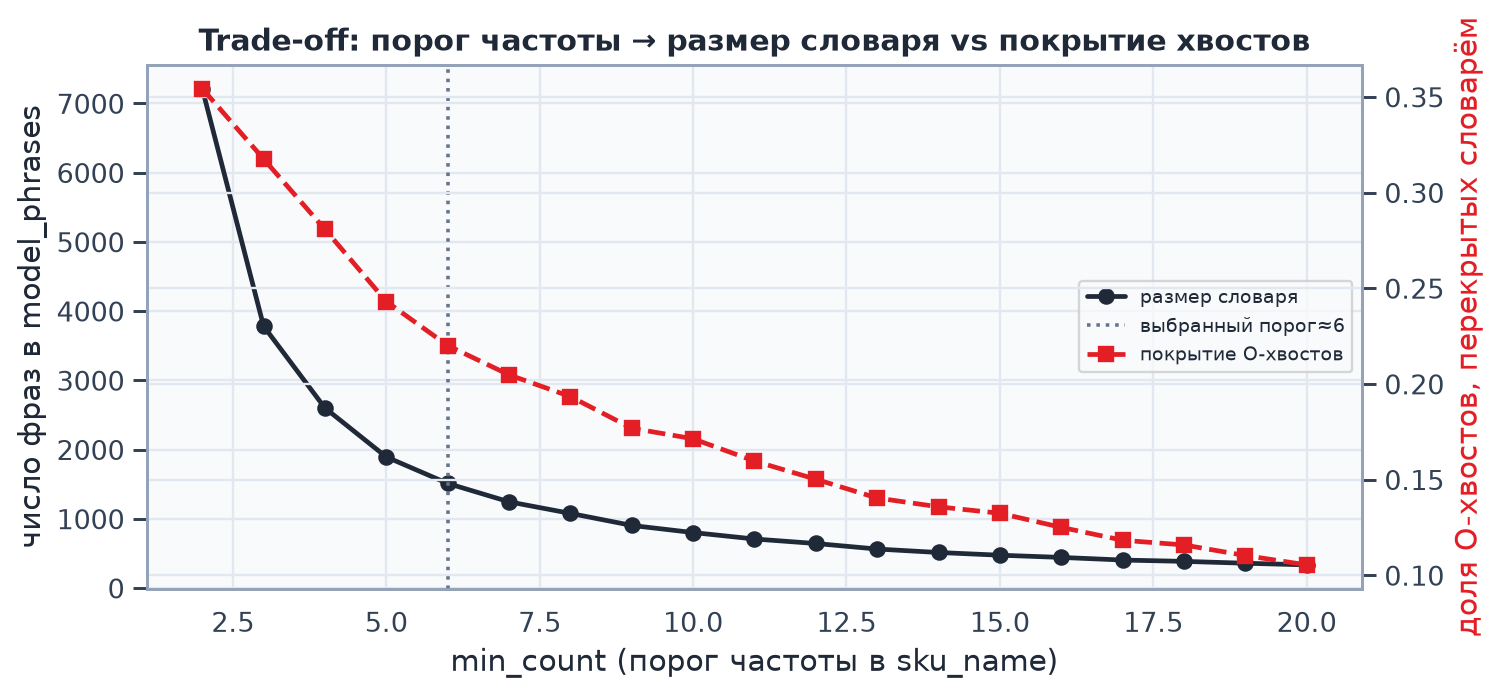
\includegraphics[width=0.98\textwidth,height=4.4cm,keepaspectratio]{model_tag/03_threshold_tradeoff.png}
\column{0.47\textwidth}
\graynote{КАК ЧИТАТЬ ГРАФИК}{Чёрная кривая — размер словаря, красная — доля хвостов, которые он покрывает. Пунктир — наш выбор.}
\vspace{6pt}\par
{\smalltext
\numdot{1}\ Из 47 тысяч названий карточек намайнили 8540 сырых кандидатов: galaxy, iphone, watch, redmi и другие.\par\vspace{4pt}
\numdot{2}\ Кривые расходятся плавно, «локтя» нет — выбрали порог 6 как компромисс между размером и покрытием.\par\vspace{4pt}
\numdot{3}\ Дополнительные фильтры: голые числа не берём; фразы из одного токена — только коды вида «v15», «g305», «ps5».}
\end{columns}
\slidefoot
\end{frame}

% ============================================================
% 13. ДО / ПОСЛЕ СЛОВАРЯ
% ============================================================
\begin{frame}[t]
\slidehead{тег model · результат}{До и после подключения словаря}
\begin{columns}[T]
\column{0.5\textwidth}
\vspace{2pt}\centering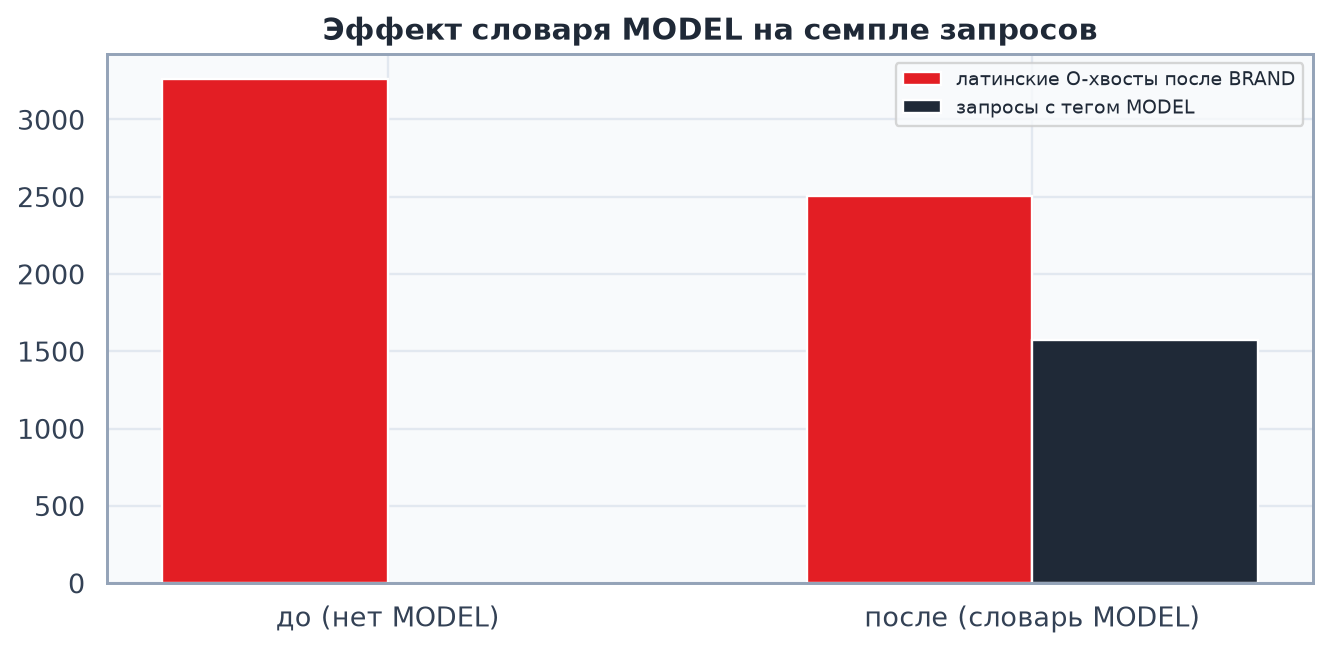
\includegraphics[width=0.98\textwidth,height=4.4cm,keepaspectratio]{model_tag/04_before_after_model_tag.png}
\column{0.47\textwidth}
\conclusion{Словарь линеек включает класс MODEL: было 0 запросов с тегом — стало 1573. Потерянных хвостов стало меньше на четверть.}
\vspace{6pt}\par
{\smalltext
\numdot{1}\ Латинские хвосты без тега: 3262 $\to$ 2502, минус 23\%.\par\vspace{4pt}
\numdot{2}\ Проверили качество словаря вручную: 96{,}6\% фраз — настоящие линейки, остальное — длинные артикулы и аксессуары, их вычистим.\par\vspace{4pt}
\numdot{3}\ Оставшиеся хвосты словарём не закрыть — это кандидаты на ручную разметку, для неё мы сделали приложение (покажем дальше).}
\end{columns}
\slidefoot
\end{frame}

% ============================================================
% 14. СХЕМЫ РАЗМЕТКИ — ТАБЛИЦА
% ============================================================
\begin{frame}[t]
\slidehead{разметка · схемы}{Какие бывают схемы токен-разметки}
\graynote{КОНТЕКСТ}{Задача NER — найти спаны сущностей. Но модели классифицируют токены, поэтому спаны кодируют в токен-схему. Разные схемы — разные способы обозначить границы.}
\vspace{6pt}\par
{\renewcommand{\arraystretch}{1.3}\setlength{\tabcolsep}{6pt}
\begin{tabular}{|L{2.0cm}|C{2.3cm}|L{7.3cm}|}
\hline
\theadl{Схема} & \thead{Теги} & \theadl{Суть}\\
\hline
\tcelll{\hb{IO}} & \tcellc{I, O} & \tcelll{самое простое, но две соседние сущности сливаются}\\
\hline
\tcelll{\hb{BIO (IOB)}} & \tcellc{B, I, O} & \tcelll{B отмечает начало — границы видны; стандарт CoNLL}\\
\hline
\tcelll{\hb{IOE}} & \tcellc{I, O, E} & \tcelll{то же самое, только отмечается конец, а не начало}\\
\hline
\tcelll{\hb{BILOU}} & \tcellc{B, I, L, O, U} & \tcelll{добавляются теги конца (L) и одиночного слова (U)}\\
\hline
\tcelll{\hb{BIES}} & \tcellc{B, I, E, S, O} & \tcelll{максимум классов — сильнее дисбаланс, учить труднее}\\
\hline
\end{tabular}}
\vspace{4pt}\par
\tnote{Общая беда всех токен-схем: вложенные сущности не выразить — «адрес» нельзя разбить на город, улицу и дом одновременно.}
\slidefoot
\end{frame}

% ============================================================
% 15. СХЕМЫ — ВЫБОР + ПРИМЕР
% ============================================================
\begin{frame}[t]
\slidehead{разметка · выбор}{Храним спаны, учим на BIO}
\conclusion{Спаны — универсальный формат хранения и оценки: любой модельный ответ приводится к ним. BIO — формат обучения. Держим оба.}
\vspace{8pt}\par
\begin{columns}[T]
\column{0.5\textwidth}
{\InterSemi\fontsize{8.5}{10.5}\selectfont Почему именно BIO}\par\vspace{5pt}
{\smalltext
\numdot{1}\ Классы — полные теги (B-BRAND, I-ATTR и так далее). Буквы B, I, O лишь кодируют границы.\par\vspace{4pt}
\numdot{2}\ У 27\% запросов сущности длиннее одного токена. Схема IO склеила бы соседние сущности в одну, BIO их разделяет.\par\vspace{4pt}
\numdot{3}\ BILOU на коротких запросах даёт больше классов без выигрыша — дисбаланс растёт, качество нет.\par\vspace{4pt}
\numdot{4}\ Наши теги: BRAND, MODEL, CATEGORY, ATTR (с приставками B и I) плюс O.}
\column{0.47\textwidth}
\begin{tikzpicture}
\node[fill=cardbg, rounded corners=3pt, inner sep=8pt, text width=\dimexpr\textwidth-16pt\relax]{
{\InterSemi\fontsize{8}{10}\selectfont Пример BIO-разметки}\par\vspace{6pt}
{\fontsize{8}{13}\selectfont\color{mvdark}
ноутбук \ \biotag{mvred}{B-CATEGORY}\par\vspace{3pt}
asus \ \biotag{mvdark}{B-BRAND}\par\vspace{3pt}
zenbook \ \biotag{okgreen}{B-MODEL}\par\vspace{3pt}
16 \ \biotag{warnorange}{B-ATTR}\par\vspace{3pt}
гб \ \biotag{warnorange}{I-ATTR}}
};
\end{tikzpicture}
\end{columns}
\slidefoot
\end{frame}

% ============================================================
% 16. НОВЫЙ: FUSION-СХЕМА — ОТКУДА БЕРЁТСЯ РАЗМЕТКА
% ============================================================
\begin{frame}[t]
\slidehead{разметка · источники}{Два сигнала сливаются в одну разметку}
\pinknote{ИДЕЯ}{Текст запроса и поведение пользователей — независимые источники правды. Их слияние даёт разметку, которой не было ни в одном из них по отдельности.}
\vspace{14pt}\par
\begin{columns}[T]
\column{0.5\textwidth}
\begin{center}
\begin{tikzpicture}[
  enc/.style={fill=cardbg, rounded corners=3pt, minimum height=1.05cm, text width=2.6cm, align=center, font=\InterSemi\fontsize{8}{9.5}\selectfont, text=mvdark},
  fus/.style={fill=mvred, rounded corners=3pt, minimum height=1.5cm, text width=2.2cm, align=center, font=\InterBold\fontsize{8.5}{10}\selectfont, text=white},
  ln/.style={mvgray, line width=0.9pt}
]
  \node[enc] (t) at (0,1.15) {Текст запроса\\{\fontsize{6.5}{8}\selectfont словари · регулярки}};
  \node[enc] (k) at (0,-1.15) {Клики\\{\fontsize{6.5}{8}\selectfont какой товар выбрали}};
  \node[fus] (f) at (4.1,0) {Слабая\\разметка};
  \draw[ln] (t.east) -- (f.west|-t.east);
  \draw[ln] (k.east) -- (f.west|-k.east);
\end{tikzpicture}
\end{center}
\column{0.47\textwidth}
{\renewcommand{\arraystretch}{1.25}\setlength{\tabcolsep}{6pt}
\begin{tabular}{|L{2.4cm}|L{3.6cm}|}
\hline
\theadl{Факт} & \theadl{Откуда сигнал}\\
\hline
\tcelll{Бренд в тексте} & \tcelll{словарь по запросу}\\
\hline
\tcelll{Скрытый бренд} & \tcelll{только клики}\\
\hline
\tcelll{Категория} & \tcelll{словарь + клики}\\
\hline
\tcelll{Модель} & \tcelll{майнинг названий карточек}\\
\hline
\tcelll{Атрибуты} & \tcelll{регулярки по тексту}\\
\hline
\end{tabular}}
\par\vspace{6pt}
{\smalltext\color{mvgray} Пример: в запросе «айфон 15 про» словарь бренда молчит, но клики говорят — Apple. А «128 гб» видит только регулярка.}
\end{columns}
\slidefoot
\end{frame}

% ============================================================
% 17. КАСКАД (шевроны как в М.Тех, всё по-русски)
% ============================================================
\begin{frame}[t]
\slidehead{mvp · архитектура}{Гибридный каскад: что уже собрано}
\pinknote{КАК УСТРОЕНО}{Каждый слой закрывает слабость предыдущего: правила — мгновенные, CRF понимает морфологию, классификатор достаёт скрытый бренд, цепь определяет тип атрибута. На выходе — факты за десятки миллисекунд.}
\vspace{20pt}\par
\begin{center}
\begin{tikzpicture}[node distance=0pt]
  \node (a) {\pipestep{mvred}{white}{ЗАПРОС\\\fontsize{6}{7}\selectfont «ноутбук asus 16 гб»}};
  \node[right=3pt of a] (c1) {\chevron};
  \node[right=3pt of c1] (b) {\pipestep{cardbg}{mvdark}{ПРАВИЛА\\\fontsize{6}{7}\selectfont словари · регулярки · модели}};
  \node[right=3pt of b] (c2) {\chevron};
  \node[right=3pt of c2] (d) {\pipestep{cardbg}{mvdark}{CRF\\\fontsize{6}{7}\selectfont разметка последовательности}};
  \node[right=3pt of d] (c3) {\chevron};
  \node[right=3pt of c3] (e) {\pipestep{cardbg}{mvdark}{КЛАССИФИКАТОР\\\fontsize{6}{7}\selectfont бренд, если не написан}};
  \node[right=3pt of e] (c4) {\chevron};
  \node[right=3pt of c4] (f) {\pipestep{mvdark}{white}{ТИПИЗАТОР\\\fontsize{6}{7}\selectfont марковская цепь}};
\end{tikzpicture}
\end{center}
\vspace{20pt}\par
\begin{center}
\begin{tikzpicture}
  \node[fill=pinkband, rounded corners=3pt, inner xsep=10pt, inner ysep=6pt,
        text width=\dimexpr\textwidth-40pt\relax, align=left] {%
    {\color{mvred}\InterBold\fontsize{8}{10}\selectfont ПЕТЛЯ КАЧЕСТВА}\hspace{7pt}%
    {\color{mvdark}\fontsize{8}{11}\selectfont неуверенные ответы и ошибки уходят в ручную разметку, на ней дообучаем CRF и пополняем словари}};
\end{tikzpicture}
\end{center}
\slidefoot
\end{frame}

% ============================================================
% 18. ПРОДАКШЕН-ПАЙПЛАЙН (наш кейс: путь запроса)
% ============================================================
\begin{frame}[t]
\slidehead{продакшен · путь запроса}{Путь запроса от строки до выдачи}
\graynote{ЗАЧЕМ}{Извлечь факты — только середина пути: дальше нормализация, каталог и ранжирование.}
\vspace{5pt}\par
\begin{center}
\begin{tikzpicture}[node distance=0pt]
  \node (p1) {\pipestepq{cardbg}{mvdark}{Запрос}};
  \node[right=2.5pt of p1] (a1) {\chevron};
  \node[right=2.5pt of a1] (p2) {\pipestepq{cardbg}{mvdark}{Пред-\\обработка}};
  \node[right=2.5pt of p2] (a2) {\chevron};
  \node[right=2.5pt of a2] (p3) {\pipestepq{mvred}{white}{Извлечение\\фактов}};
  \node[right=2.5pt of p3] (a3) {\chevron};
  \node[right=2.5pt of a3] (p4) {\pipestepq{cardbg}{mvdark}{Нормали-\\зация}};
  \node[right=2.5pt of p4] (a4) {\chevron};
  \node[right=2.5pt of a4] (p5) {\pipestepq{cardbg}{mvdark}{Каталог}};
  \node[right=2.5pt of p5] (a5) {\chevron};
  \node[right=2.5pt of a5] (p6) {\pipestepq{cardbg}{mvdark}{Ранжиро-\\вание}};
\end{tikzpicture}
\end{center}
\vspace{5pt}\par
{\renewcommand{\arraystretch}{1.1}\setlength{\tabcolsep}{7pt}
\begin{center}
\begin{tabular}{|L{3.2cm}|L{8.4cm}|}
\hline
\theadl{Шаг} & \theadl{Пример}\\
\hline
\tcelll{\hb{Нормализация}} & \tcelll{«16гб», «16 gb», «16 ГБ» — всё превращается в одно значение: 16 ГБ}\\
\hline
\tcelll{\hb{Каталог}} & \tcelll{категория «ноутбук» находит узел «Ноутбуки и планшеты»}\\
\hline
\tcelll{\hb{Ранжирование}} & \tcelll{карточки с брендом asus и памятью 16 ГБ идут наверх}\\
\hline
\end{tabular}
\end{center}}
\vspace{-2pt}
\slidefoot
\end{frame}

% ============================================================
% 19. КЛАССИФИКАТОР БРЕНДА
% ============================================================
\begin{frame}[t]
\slidehead{mvp · классификатор бренда}{Бренд, когда его нет в тексте}
\graynote{НА ЧЁМ УЧИЛИ}{Обучающее множество собрано автоматически из кликов: запрос $\to$ самый частый бренд среди кликнутых карточек. Ни одной ручной метки.}
\vspace{8pt}\par
\begin{columns}[T]
\column{0.5\textwidth}
{\InterSemi\fontsize{8.5}{10.5}\selectfont Как устроен}\par\vspace{5pt}
{\smalltext
\numdot{1}\ Признаки — кусочки слов по 3–5 букв. Поэтому «айфон», «afon» и «iphone» выглядят похоже, опечатки не страшны.\par\vspace{4pt}
\numdot{2}\ 18 914 обучающих запросов, сорок самых частых брендов.\par\vspace{4pt}
\numdot{3}\ Включается только когда словарь не нашёл бренд в тексте — как запасной вариант.}
\column{0.47\textwidth}
{\InterSemi\fontsize{8.5}{10.5}\selectfont Быстрый тест}\par\vspace{5pt}
\begin{tikzpicture}[st/.style={rounded corners=2pt, fill=cardbg, inner sep=6pt, text width=\dimexpr\textwidth-14pt\relax, font=\smalltext}]
\node[st]{
\begin{tabular}{@{}ll@{}}
Точность (топ-40 брендов) & \InterBold\color{mvred}0{,}80\\[3pt]
Средний F1 по классам & \InterBold\color{mvred}0{,}77\\[3pt]
Обучающих запросов & \InterBold 18 914\\
\end{tabular}};
\end{tikzpicture}
\par\vspace{6pt}
{\fontsize{8}{12}\selectfont
\wplain{айфон 15 про макс} \ \chevron\ \wtag{mvdark}{Apple}\par\vspace{3pt}
\wplain{редми ноут 13} \ \chevron\ \wtag{mvdark}{Xiaomi}}
\end{columns}
\slidefoot
\end{frame}

% ============================================================
% 20. CRF
% ============================================================
\begin{frame}[t]
\slidehead{mvp · crf}{CRF на слабой разметке, путь к золотой}
\pinknote{ЧЕСТНОСТЬ}{Числа ниже — проверка «повторила ли модель правила», поэтому они завышены. Настоящую оценку даст только ручная золотая разметка.}
\vspace{8pt}\par
\begin{columns}[T]
\column{0.44\textwidth}
{\InterSemi\fontsize{8.5}{10.5}\selectfont Быстрый тест на выборке}\par\vspace{5pt}
\begin{tikzpicture}[st/.style={rounded corners=2pt, fill=cardbg, inner sep=6pt, text width=\dimexpr\textwidth-14pt\relax, font=\smalltext}]
\node[st]{
\begin{tabular}{@{}ll@{}}
Точность по токенам & \InterBold\color{mvred}0{,}91\\[3pt]
F1 по сущностям & \InterBold\color{mvred}0{,}875\\[3pt]
F1 бренды & \InterBold 0{,}95\\[3pt]
F1 категории & \InterBold 0{,}82\\[3pt]
F1 атрибуты & \InterBold 0{,}85\\
\end{tabular}};
\end{tikzpicture}
\column{0.54\textwidth}
{\InterSemi\fontsize{8.5}{10.5}\selectfont Слабая и золотая разметка}\par\vspace{5pt}
{\smalltext
\numdot{1}\ Слабая — автоматическая, от словарей и правил: много и бесплатно, но с шумом. На ней учим.\par\vspace{4pt}
\numdot{2}\ Золотая — ручная, 300–1000 запросов со спанами моделей. На ней честно меряем.\par\vspace{4pt}
\numdot{3}\ Если и учить, и проверять на одних и тех же автоматических метках — модель просто копирует правила, а числа льстят. Отложенная золотая выборка решает это.\par\vspace{4pt}
\numdot{4}\ Дальше: переобучить CRF на разметке с тегом MODEL и свериться с золотой.}
\end{columns}
\slidefoot
\end{frame}

% ============================================================
% 21. МАРКОВСКИЕ ЦЕПИ + ПРИМЕР
% ============================================================
\begin{frame}[t]
\slidehead{mvp · марковские цепи}{Тип атрибута: «16 гб» — это память}
\begin{columns}[T]
\column{0.5\textwidth}
\vspace{2pt}\centering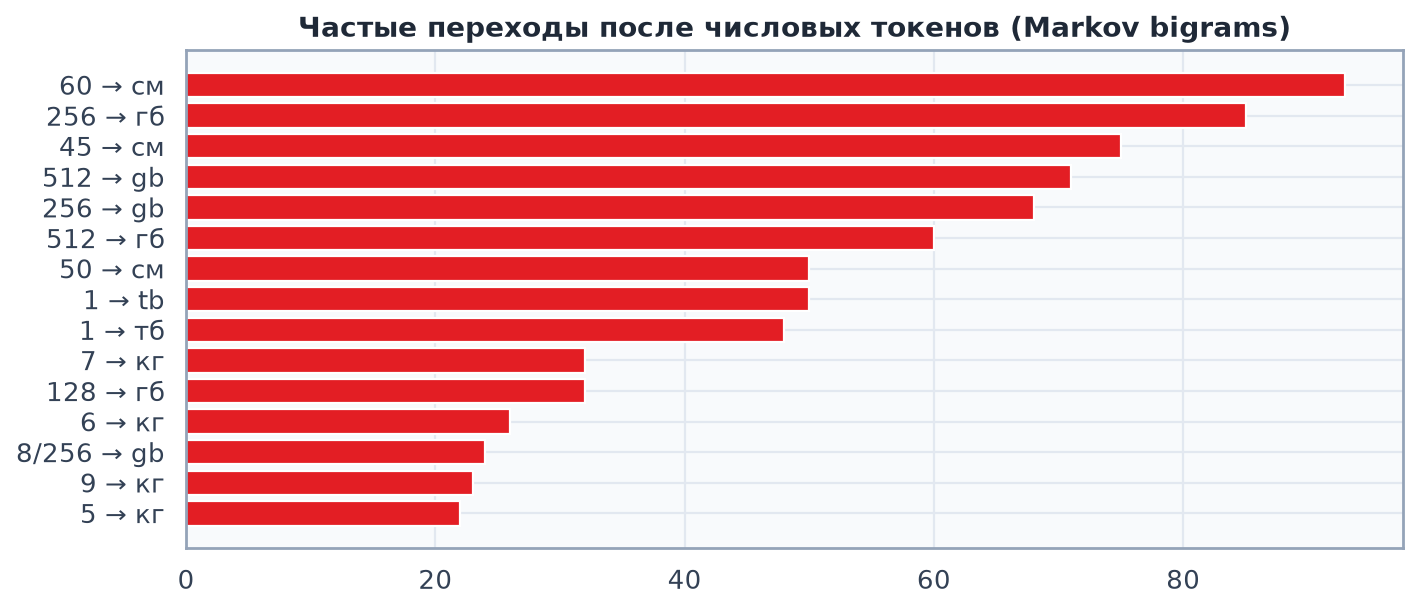
\includegraphics[width=0.98\textwidth,height=4.4cm,keepaspectratio]{markov/03_markov_transitions.png}
\column{0.47\textwidth}
\graynote{КАК РАБОТАЕТ}{CRF находит спан атрибута, а марковская цепь по паре соседних токенов говорит его тип: после «256» почти всегда идёт «гб» — значит это память.}
\vspace{6pt}\par
{\fontsize{8}{12}\selectfont
\wtag{warnorange}{16 гб} \ \chevron\ \wplain{память}\qquad
\wtag{warnorange}{55 дюймов} \ \chevron\ \wplain{диагональ}\par\vspace{3pt}
\wtag{warnorange}{2 кг} \ \chevron\ \wplain{вес}\qquad
\wtag{warnorange}{wi-fi} \ \chevron\ \wplain{связь}}
\par\vspace{6pt}
{\smalltext
\numdot{1}\ Это таблица частот, выученная из данных, — никакой нейросети. Ответ за доли миллисекунды.\par\vspace{4pt}
\numdot{2}\ Точность против правил-учителя — 0{,}62; в 36\% случаев цепь честно говорит «не знаю», но почти никогда не путает типы между собой.\par\vspace{4pt}
\numdot{3}\ Готовый обученный модуль лежит в репозитории: обучение на слабой разметке одной командой.}
\end{columns}
\slidefoot
\end{frame}

% ============================================================
% 22. МАРКОВ — ГРАНИЦА МЕТОДА
% ============================================================
\begin{frame}[t]
\slidehead{mvp · границы метода}{Где цепь бессильна: голое число}
\begin{columns}[T]
\column{0.5\textwidth}
\vspace{2pt}\centering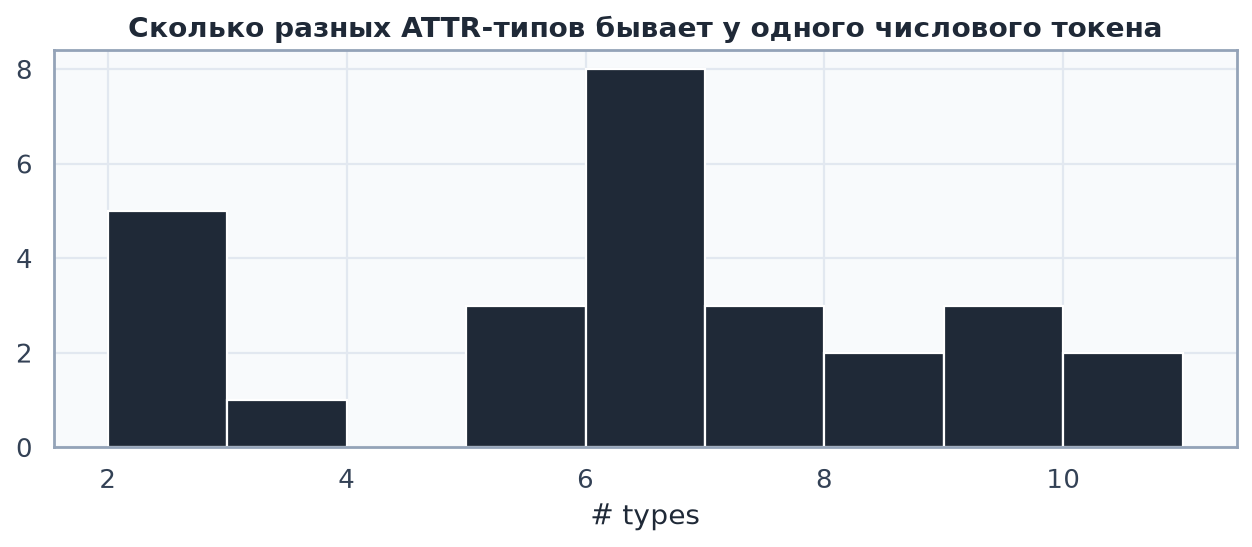
\includegraphics[width=0.98\textwidth,height=4.4cm,keepaspectratio]{markov/05_number_ambiguity.png}
\column{0.47\textwidth}
\pinknote{ПРЕДЕЛ}{Число без единицы измерения многозначно: «5» встречается в десяти разных типах атрибутов. Пара токенов тут не помогает — нужен контекст категории.}
\vspace{6pt}\par
{\smalltext
\numdot{1}\ Нашли 27 «числовых омонимов»: «5» и «12» бывают десятью разными атрибутами, «1» — восемью.\par\vspace{4pt}
\numdot{2}\ План усложнения по лестнице: правила $\to$ цепь $\to$ лёгкий классификатор с учётом категории $\to$ нейросеть только для омонимов.\par\vspace{4pt}
\numdot{3}\ Берём самый дешёвый слой, который держит время ответа, — и усложняем только там, где он ошибается.}
\end{columns}
\slidefoot
\end{frame}

% ============================================================
% 23. СООТВЕТСТВИЕ 1/0
% ============================================================
\begin{frame}[t]
\slidehead{разметка · соответствие 1/0}{Чистим шумные клики моделью}
\graynote{ЗАЧЕМ}{Клик — шумный сигнал: пользователь искал айфон, а кликнул чехол. Такие пары портят обучение. Убираем их бинарной моделью «соответствует или нет».}
\vspace{10pt}\par
\begin{center}
\begin{tikzpicture}[node distance=0pt]
  \node (m1) {\pipestep{cardbg}{mvdark}{Ручная разметка\\\fontsize{6}{7}\selectfont 100+ пар}};
  \node[right=3pt of m1] (mc1) {\chevron};
  \node[right=3pt of mc1] (m2) {\pipestep{mvred}{white}{Обучаем модель\\\fontsize{6}{7}\selectfont бустинг}};
  \node[right=3pt of m2] (mc2) {\chevron};
  \node[right=3pt of mc2] (m3) {\pipestep{cardbg}{mvdark}{Модель метит\\\fontsize{6}{7}\selectfont миллионы пар: 1 / 0}};
  \node[right=3pt of m3] (mc3) {\chevron};
  \node[right=3pt of mc3] (m4) {\pipestep{cardbg}{mvdark}{Где 1 — берём\\\fontsize{6}{7}\selectfont карточку в выдачу}};
\end{tikzpicture}
\end{center}
\vspace{12pt}\par
\begin{columns}[T]
\column{0.5\textwidth}
{\InterSemi\fontsize{8.5}{10.5}\selectfont Пример пары}\par\vspace{5pt}
{\fontsize{8}{12}\selectfont
\wplain{ноутбук asus 16} \ + \ \wplain{ASUS VivoBook 16} \ \chevron\ \wtag{okgreen}{1}\par\vspace{4pt}
\wplain{ноутбук asus 16} \ + \ \wplain{Чехол для MacBook} \ \chevron\ \wtag{mvred}{0}}
\column{0.47\textwidth}
{\smalltext
\numdot{1}\ Признаки: похожесть текста запроса и названия, совпадение бренда, позиция клика.\par\vspace{4pt}
\numdot{2}\ Дальше доразмечаем только пары, где модель сомневается, — так разметка окупается быстрее.}
\end{columns}
\slidefoot
\end{frame}

% ============================================================
% 24. СТРАТЕГИЯ РАЗМЕТКИ (цикл, как в шаблоне М.Тех)
% ============================================================
\begin{frame}[t]
\slidehead{разметка · стратегия}{Данные и стратегия разметки}
\pinknote{ПРИНЦИП}{Разметку проектируем, а не «докупаем объёмом»: размечаем в первую очередь то, на чём модель ошибается или сомневается.}
\vspace{10pt}\par
\begin{columns}[T]
\column{0.42\textwidth}
\begin{center}
\begin{tikzpicture}[
  bx/.style={rounded corners=3pt, minimum height=0.85cm, text width=2.0cm, align=center, font=\InterSemi\fontsize{8}{9.5}\selectfont},
  ar/.style={-{Stealth[length=2.4mm]}, line width=1.3pt, mvred}
]
  \node[bx, fill=mvdark, text=white] (model) at (0,1.3) {Модель};
  \node[bx, fill=mvred, text=white] (unc) at (2.3,0) {Сомнения};
  \node[bx, fill=mvdark, text=white] (lab) at (0,-1.3) {Разметка};
  \node[bx, fill=mvred, text=white] (ret) at (-2.3,0) {Дообучение};
  \draw[ar] (model.south east) to[bend left=25] (unc.north);
  \draw[ar] (unc.south) to[bend left=25] (lab.north east);
  \draw[ar] (lab.north west) to[bend left=25] (ret.south);
  \draw[ar] (ret.north) to[bend left=25] (model.south west);
\end{tikzpicture}
\end{center}
\column{0.55\textwidth}
{\smalltext
\numdot{1}\ {\InterSemi Активное обучение.} Размечаем то, в чём модель не уверена, — каждая метка приносит максимум пользы.\par\vspace{4pt}
\numdot{2}\ {\InterSemi Слабая разметка.} Правила и словари дают дешёвые метки — миллионы примеров без человека.\par\vspace{4pt}
\numdot{3}\ {\InterSemi Помощь разметчику.} Приложение показывает готовые подсказки — человек правит, а не размечает с нуля.\par\vspace{4pt}
\numdot{4}\ {\InterSemi Золотые наборы.} Эталон для честной оценки и контроля дрейфа. Первая волна — 3$\times$1500 запросов на троих.}
\end{columns}
\slidefoot
\end{frame}

% ============================================================
% 25. ПРИЛОЖЕНИЕ РАЗМЕТКИ — СКРИНШОТЫ
% ============================================================
\begin{frame}[t]
\slidehead{приложение · разметка}{Готово: приложение для разметки команды}
\graynote{ТРИ СБОРКИ}{Для Никиты, Некита и Лизы — по 1500 уникальных запросов, наборы не пересекаются. Клавиши B, I, O + выбор категории, история с правкой, прогресс и автосохранение в файл.}
\vspace{8pt}\par
\begin{columns}[T]
\column{0.49\textwidth}
\centering
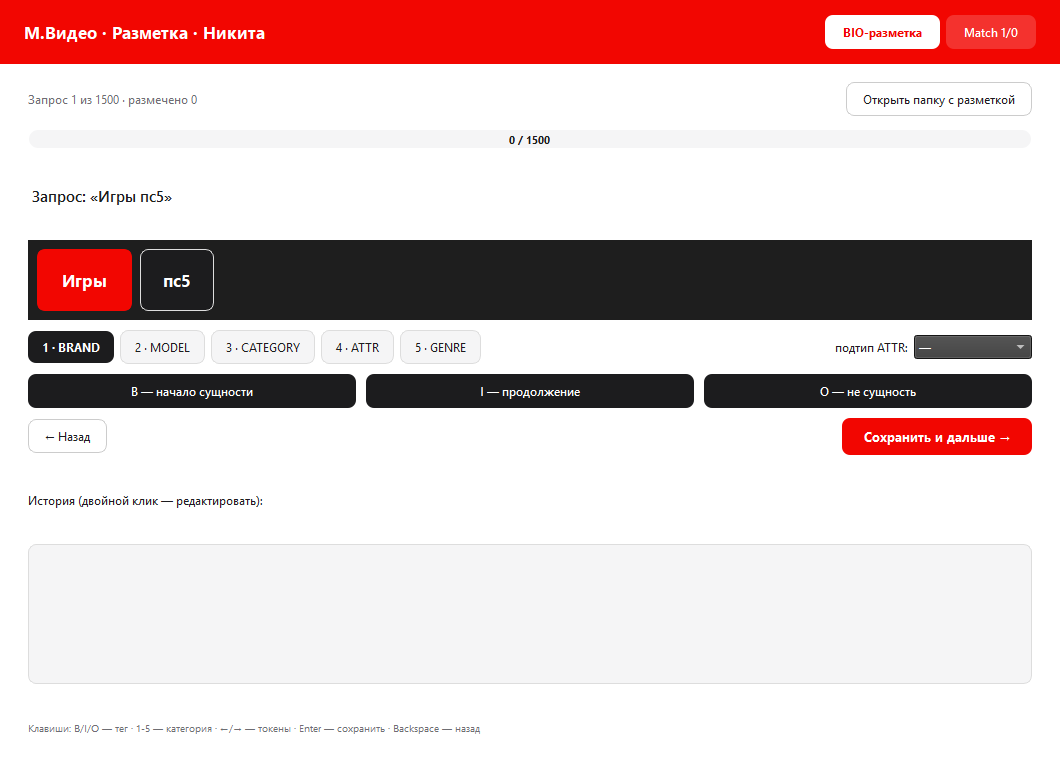
\includegraphics[width=\textwidth]{apps/labeling_bio.png}\par\vspace{3pt}
{\smalltext\color{mvgray} Режим BIO: токены-кнопки, категории 1–5, подтип атрибута}
\column{0.49\textwidth}
\centering
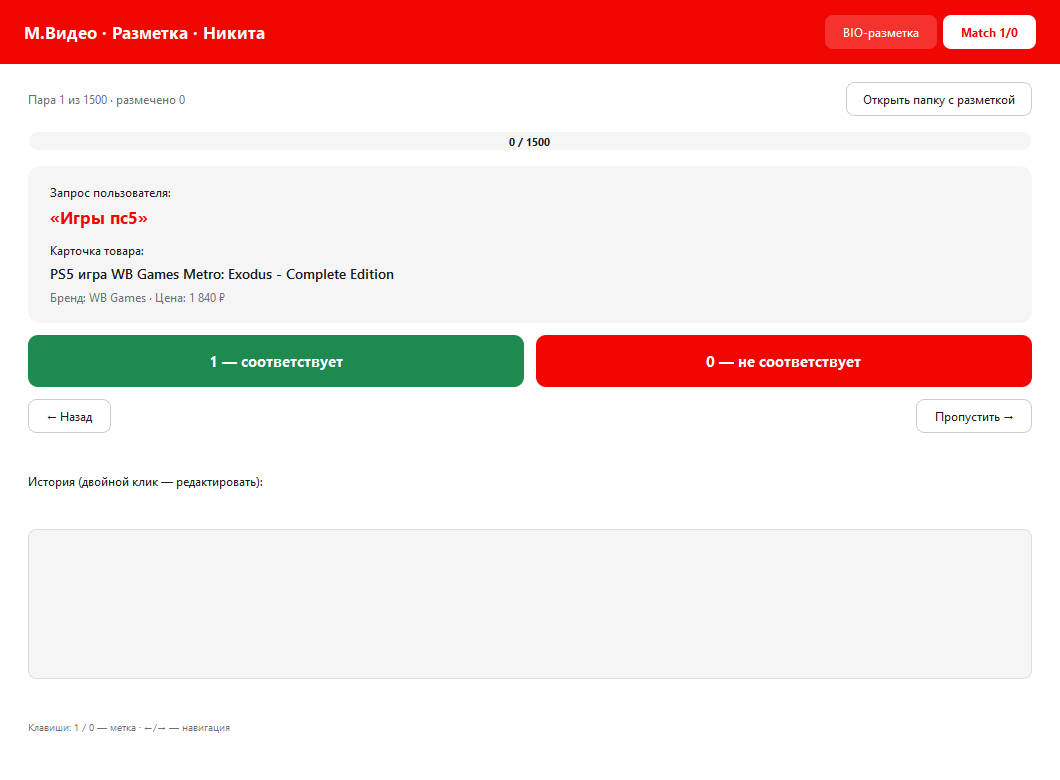
\includegraphics[width=\textwidth]{apps/labeling_match.png}\par\vspace{3pt}
{\smalltext\color{mvgray} Режим 1/0: запрос против карточки, две кнопки, отдельный файл}
\end{columns}
\slidefoot
\end{frame}

% ============================================================
% 26. MVP-ПРИЛОЖЕНИЕ — СКРИНШОТЫ
% ============================================================
\begin{frame}[t]
\slidehead{приложение · умный поиск}{Готово: MVP умного поиска}
\pinknote{КИЛЛЕР-ФИЧА}{Ранжирование каталога опирается только на извлечённые факты — бренд, категорию, модель и атрибуты, — а не на сырой текст запроса.}
\vspace{8pt}\par
\begin{columns}[T]
\column{0.49\textwidth}
\centering
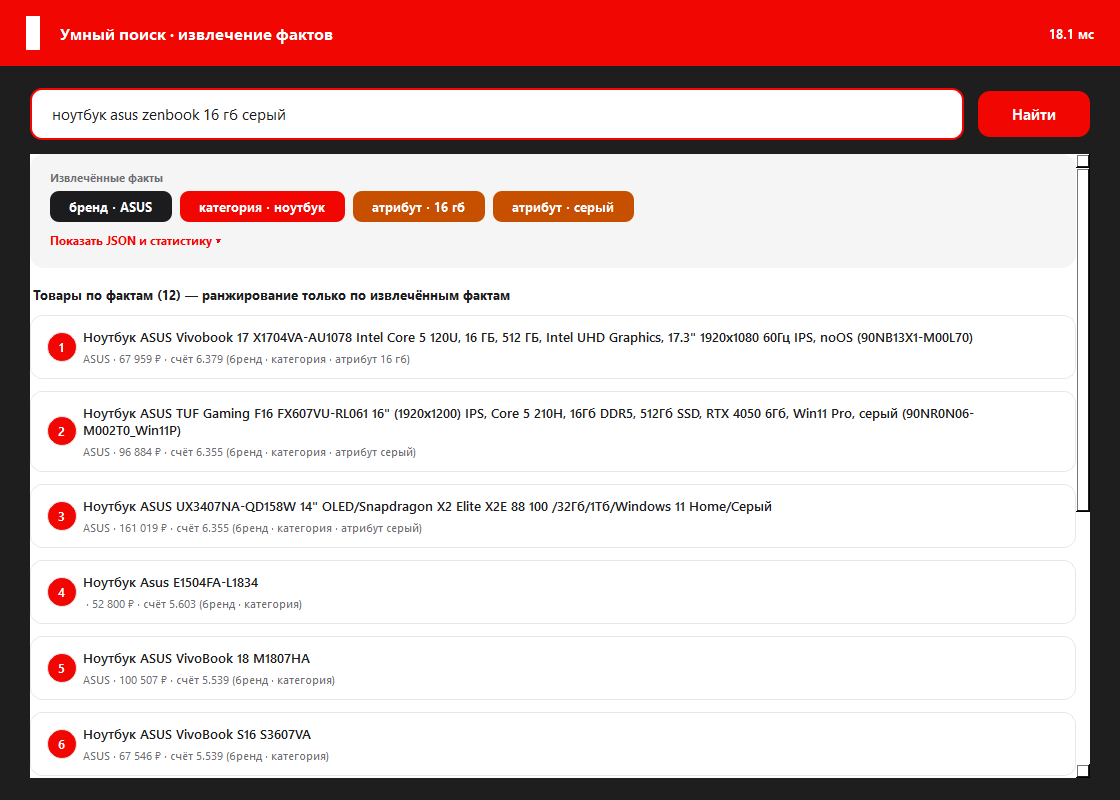
\includegraphics[width=\textwidth]{apps/mvp_search.png}\par\vspace{3pt}
{\smalltext\color{mvgray} Факты чипами + товары, отранжированные по фактам, с объяснением счёта}
\column{0.49\textwidth}
\centering
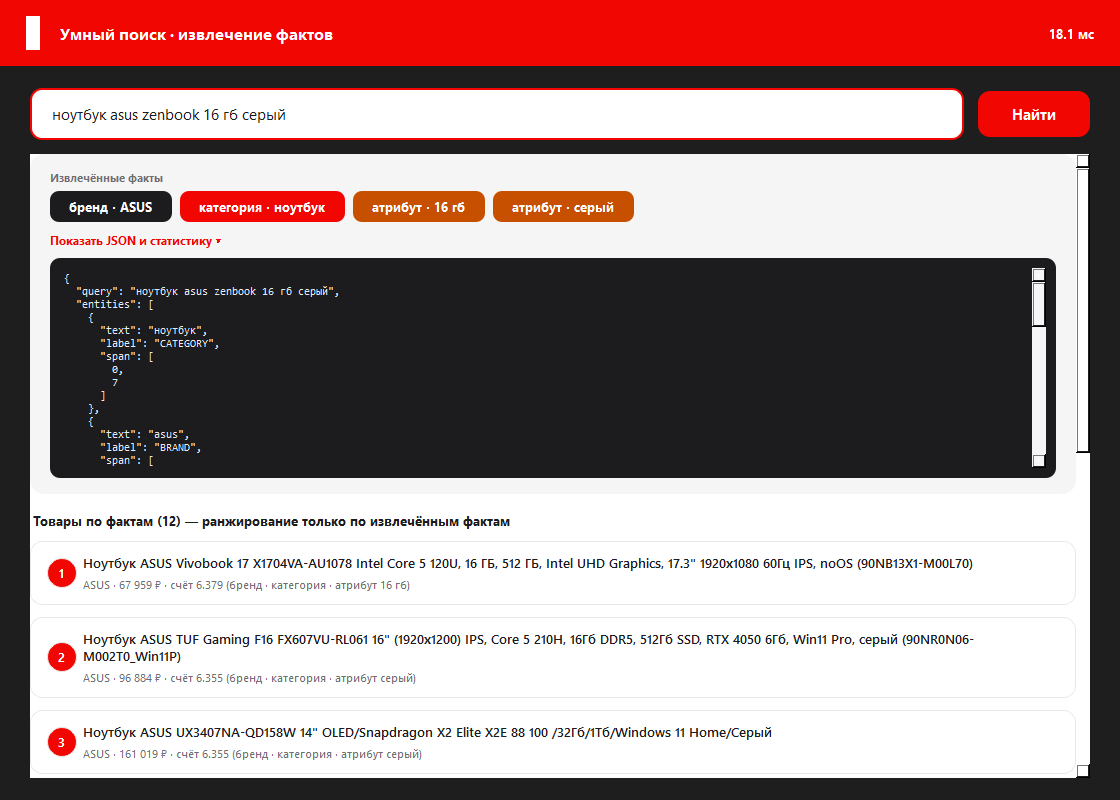
\includegraphics[width=\textwidth]{apps/mvp_json.png}\par\vspace{3pt}
{\smalltext\color{mvgray} По клику раскрывается JSON и статистика слоёв каскада; таймер — в шапке}
\end{columns}
\slidefoot
\end{frame}

% ============================================================
% 27. ДАЛЬШЕ
% ============================================================
\begin{frame}[t]
\slidehead{план · дальше}{Следующие шаги}
\begin{columns}[T]
\column{0.48\textwidth}
{\InterSemi\fontsize{8.5}{10.5}\selectfont Модели}\par\vspace{6pt}
{\smalltext
\numdot{1}\ Переобучить CRF на разметке с тегом MODEL и свериться с золотой выборкой.\par\vspace{5pt}
\numdot{2}\ Классификаторы бренда и категории на кликах, очищенных моделью соответствия.\par\vspace{5pt}
\numdot{3}\ Типизатор атрибутов: цепь, затем лёгкий классификатор с контекстом категории для омонимов.}
\column{0.48\textwidth}
{\InterSemi\fontsize{8.5}{10.5}\selectfont Данные и продукт}\par\vspace{6pt}
{\smalltext
\numdot{4}\ Команда размечает первую волну: 3$\times$1500 запросов и пары для модели соответствия.\par\vspace{5pt}
\numdot{5}\ Собранную золотую разметку — в честную оценку каскада.\par\vspace{5pt}
\numdot{6}\ Умный поиск: реранжирование с описанием карточки, больше статистики в интерфейсе.}
\end{columns}
\vspace{10pt}\par
\pinknote{ЦЕЛЬ К ЗАЩИТЕ}{Рабочий каскад с покрытием сложных случаев и честные метрики на ручной золотой разметке, а не самопроверка словаря.}
\slidefoot
\end{frame}

% ============================================================
% 28. ФИНАЛ
% ============================================================
\begin{frame}[plain]
\begin{tikzpicture}[remember picture, overlay]
  \fill[mvred] (current page.south west) rectangle (current page.north east);
  \node[anchor=east, inner sep=0pt] at ([xshift=0.32\paperwidth]current page.east)
    {
\includegraphics[height=1.06\paperheight]{kurs1_image1.png}};
  \node[anchor=west, align=left] at ([xshift=0.9cm, yshift=2.1cm]current page.west)
    {\color{white}\InterBold\fontsize{23}{27}\selectfont Спасибо!};
  \node[anchor=west, align=left, text width=0.52\paperwidth] at ([xshift=0.9cm, yshift=1.05cm]current page.west)
    {\color{white}\fontsize{9.5}{13}\selectfont MVP собран: предобработка, тег MODEL, каскад моделей и два приложения. Дальше — золотая разметка и качество.};
  \node[anchor=west, align=left, text width=0.55\paperwidth] at ([xshift=0.9cm, yshift=-0.85cm]current page.west)
    {\color{white}\fontsize{8.5}{13}\selectfont
     {\InterSemi Команда:}\\[2pt]
     Новицкий Никита · @n.novitskiy\\
     Борисов Никита · @n.borisov\\
     Засухина Елизавета · @e.zasukhina\\
     Олейников Александр · @a.oleynikov};
  \node[anchor=south west] at ([xshift=0.9cm, yshift=0.5cm]current page.south west)
    {\color{white}\fontsize{8}{10}\selectfont Презентация свёрстана в \TeX\ / \LaTeX\ · День 03 · Глубокий EDA и MVP · Буткемп М.Видео};
\end{tikzpicture}
\end{frame}

\end{document}

